
\chapter{Introduction}
\label{chapter:introduction}

\section{Section}


\lipsum[2]

\subsection{Subsection}

\lipsum[1]


%
\begin{equation}
S   = \int dt L
\end{equation}
%
\lipsum[3] 
%
\begin{equation}
\frac{d}{dt} \left( \frac{\partial L}{\partial \dot{q}_i} \right) - \frac{\partial L}{\partial q_i} = 0
\end{equation}
%
\lipsum[3]
\begin{equation}
L(t,q_i , \dot{q}_i) \rightarrow \mathcal{L}\left(x_\mu , \phi , \frac{\partial \phi}{\partial x_\mu} \right)
\end{equation}
%
\lipsum[3]
%
\begin{equation}
S = \int dt L = \int dx^4 \mathcal{L}	
\end{equation}
%
\lipsum[4]
%
\begin{equation}
\partial_\mu \left( \frac{\partial \mathcal{L}}{\partial (\partial_\mu \phi)}\right) - \frac{\partial \mathcal{L}}{\partial \phi} = 0
\end{equation}
%


\begin{figure}[ht!]
	\centering
	%   \resizebox{0.8\textwidth}{!}{
	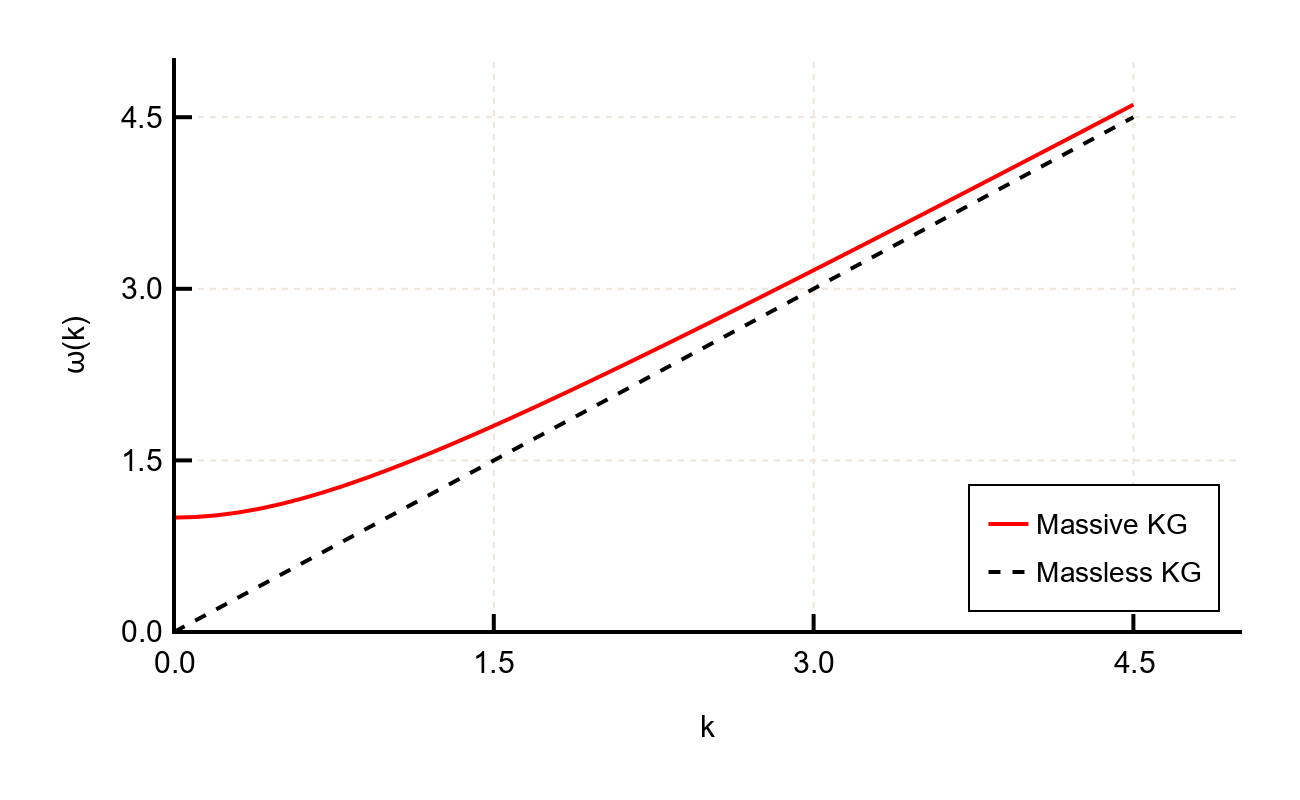
\includegraphics[width=0.8\linewidth]{figures/klein_gordon_DR}
	%    }
	\caption[Example figure 1]{ This is an example image with a caption }
	\label{fig:phasediagram_fluid}
\end{figure}




\subsection{Another Subsection}

\lipsum[1]

\subsubsection*{A Subsection without a number!}


\lipsum[3]

\begin{shaded}
	\textbf{Remark:}
	
	This is a block that can also be used for theorems, small notes...
	%
	\begin{equation}
	\eta_{\mu \nu} = ( - \;,\; + \;,\; + \;,\; +)
	\end{equation}
	
\end{shaded}

\lipsum[3]

\section{Last Section}

\lipsum[2]


\subsection{Example Table}
\lipsum[7]
%

\begin{table}[h]
\begin{center}
	\begin{tabular}{ ||p{3cm}|p{3cm}||p{3cm}|p{3cm}||  }
		\hline
		\multicolumn{4}{|c|}{\textbf{Table Title}} \\
		\hline
		\multicolumn{2}{||c||}{\textbf{Group I}} & \multicolumn{2}{c||}{\textbf{Group II}} \\
		\hline
		Parameter 1   	& 	1.0    	& Parameter 3		&   1.0	\\
		Parameter 2   	& 	27.0  	& Parameter 4   	&	0  	\\
		\hline
	\end{tabular}
  \captionsetup{width=14cm}

\caption{ An example table with a matching caption. If you change the size of the table, make sure to change the caption setup above }\label{tab:noPublications}
\end{center}
\end{table}

\lipsum[3]
\lipsum[3-5]

\begin{figure}[!hb]
	\centering
	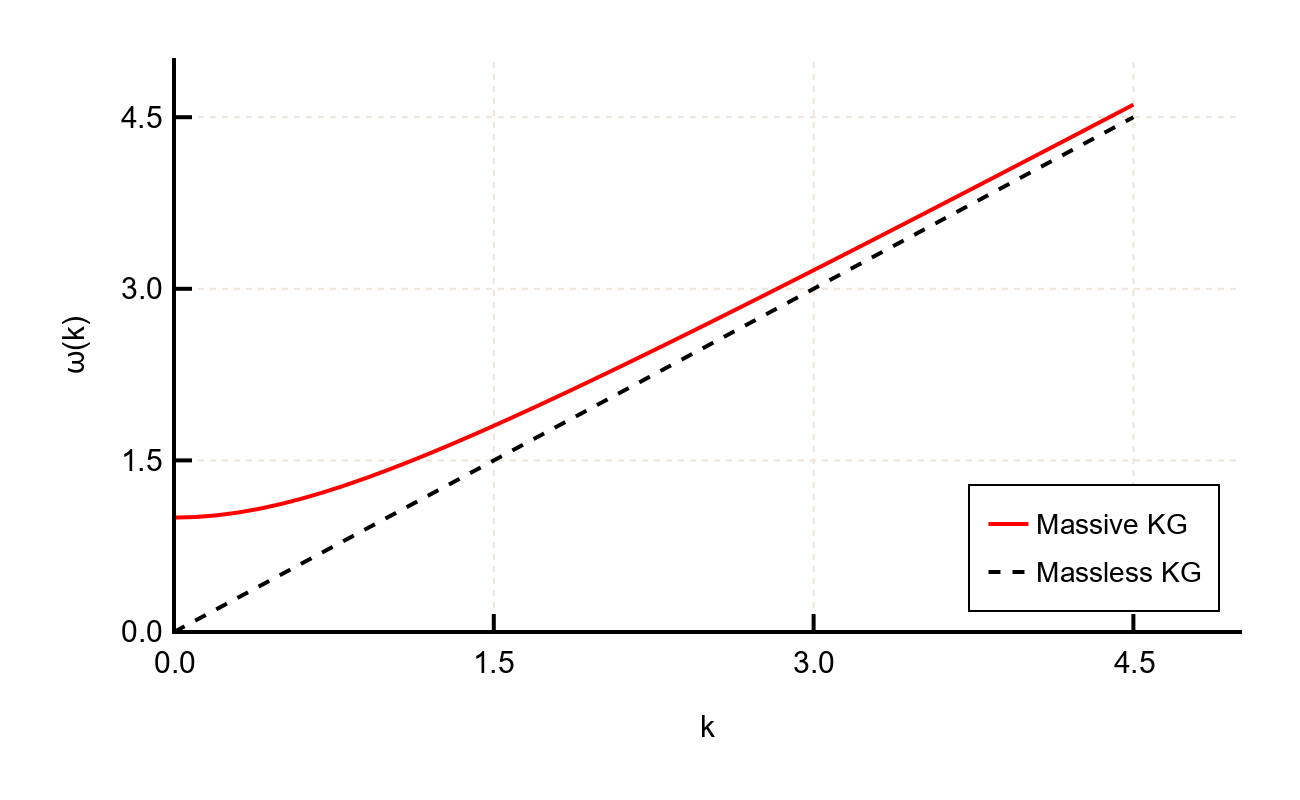
\includegraphics[width=0.8\textwidth]{figures/klein_gordon_DR}
	\caption[Example figure 2]{This is another example image with a longer caption. If the text is too long it wraps automatically underneath the figure. }
	\label{fig:richtmyerstencil}
\end{figure}

